\documentclass[12pt]{article}
\usepackage[top=1.0in, bottom=0.6in, left=0.9in, right=1.1in]{geometry}

\usepackage{graphicx,color,enumitem}
\usepackage{amsmath,amsthm,amsbsy}
\usepackage{palatino}

\usepackage{tikz}

%% Setup aproblem environment, 
%% aproblem items
%% subproblems environment
%% subproblem items
\makeatletter
\newcounter{probcount}
\newcounter{subprobcount}
\newlength\probsep
\newlength\pshrinking
\newif\iffirstprob

\newenvironment{aproblems}%
  {\ifhmode\unskip\par\fi\setcounter{probcount}{0}\probsep\parskip
  \sbox\@tempboxa{\textbf{9.}}\pshrinking\wd\@tempboxa\advance\pshrinking\labelsep
  \let\hproblem\aproblem
  \advance\linewidth -\pshrinking
  \advance\@totalleftmargin\pshrinking
  \advance\leftskip\pshrinking}%
  {\ifhmode\unskip \par\fi\advance\leftskip-\pshrinking}%

\newcommand{\aproblem}{%
  \setcounter{subprobcount}{0}%
  \stepcounter{probcount}%
  \def\@currentlabel{\arabic{probcount}}%
  \ifhmode
    \unskip \par
  \fi
%  \addpenalty{-4000}%
  \iffirstprob\else\addvspace\probsep\fi
  \firstprobfalse
  \hskip -\labelwidth\hskip -\labelsep 
  \hbox to\labelwidth{\hss\textbf{\arabic{probcount}.}}\hskip\labelsep
}%

\newcommand{\subprob}{\item\def\@currentlabel{\arabic{probcount}\alph{\thelistlabel}}}
\newcommand{\skipproblem}{\stepcounter{probcount}}


%% The following commands put defined left and right headers on the top, and a page number
%% on the bottom of all pages beyond page 1
\usepackage{fancyhdr}
\pagestyle{fancy}
\fancyfoot[C]{\ifnum \value{page} > 1\relax\thepage\fi}
\fancyhead[L]{\ifx\@doclabel\@empty\else\@doclabel\fi}
\fancyhead[R]{\ifx\@docdate\@empty\else\@docdate\fi}
\headheight 15pt
\def\doclabel#1{\gdef\@doclabel{#1}}
\def\docdate#1{\gdef\@docdate{#1}}
\makeatother

%% General formatting parameters
\parindent 0pt
\parskip 6pt plus 1pt

\newcommand{\epart}[1]{\noindent \textbf{(#1)} \,}
\newcommand{\ds}{\displaystyle}

\doclabel{Math F302 Worksheet}
\docdate{23 October 2023}


\begin{document}
\renewcommand{\d}{\displaystyle}

\centerline{{\Large \textsc{Non-homogeneous equations (\S4.4):} \hspace{30mm}}}

\medskip
\centerline{{\Large \textsc{find $y_c$ and the form of $y_p$} \hspace{33mm}}}

\vspace{-20mm}

%\def\BEAVER{}
%\def\MOOSE{}
\def\TURTLE{}

\ifdefined\BEAVER
\hfill 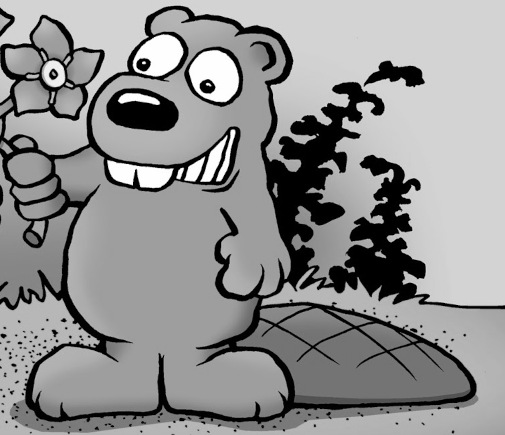
\includegraphics[height=30mm]{figs/beaver.jpg}
\else
\ifdefined\MOOSE
\hfill 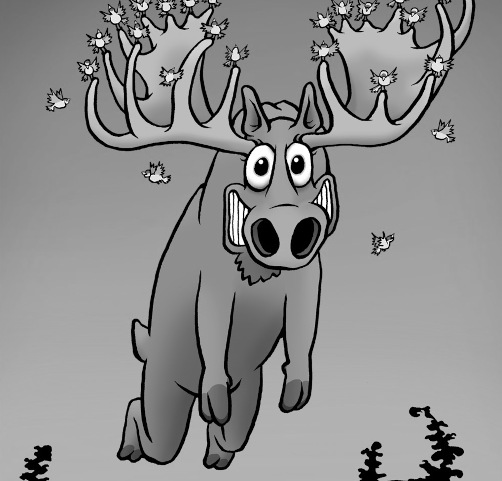
\includegraphics[height=30mm]{figs/moose.jpg}
\else
\hfill 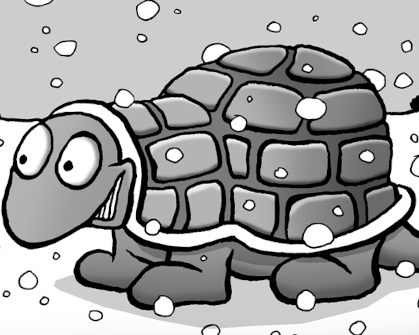
\includegraphics[height=30mm]{figs/turtle.jpg}
\fi
\fi

\medskip
\noindent
Team effort!  For each differential equation, find the complementary function $y_c(x)$, the general solution of the associated homogeneous equation.  Then write down the correct form for $y_p(x)$, the particular solution.  You do not need to find the unknown constants in $y_p(x)$, but you must identify the correct form, whether in case I (\emph{no duplication of terms in $y_c(x)$}) or in case II (\emph{with duplication}).  Feel free to use the table at the bottom of the page.

\bigskip

\begin{aproblems}
\ifdefined\BEAVER
\aproblem \quad $\ds y'' + 9 y = x + 2$
\else
\ifdefined\MOOSE
\aproblem \quad $\ds y'' + 4 y = 3 x + 3$
\else
\aproblem \quad $\ds y'' + 16 y = 5 - x$
\fi
\fi
\vfill

\ifdefined\BEAVER
\aproblem \quad $\ds y'' - 3 y' - 4 y = 17 e^{4x}$
\else
\ifdefined\MOOSE
\aproblem \quad $\ds y'' + y' - 6 y = 41 e^{-3x}$
\else
\aproblem \quad $\ds y'' - 6 y' + 5 y = 13 e^{x}$
\fi
\fi
\vfill

\ifdefined\BEAVER
\aproblem \quad $\ds y'' + 2 y' + y = \sin 3x + 2 \cos x$
\else
\ifdefined\MOOSE
\aproblem \quad $\ds y'' - 2 y' + y = - \sin 3x - 2 \cos x$
\else
\aproblem \quad $\ds y'' - 4 y' + 4 y = 2 \sin 3x + \cos x$
\fi
\fi
\vfill

\ifdefined\BEAVER
\aproblem \quad $\ds y'' - 7 y' = x^2 + 4 x + 7$
\else
\ifdefined\MOOSE
\aproblem \quad $\ds y'' - 5 y' = 2 x^2 + 5 x + 8$
\else
\aproblem \quad $\ds y'' - 9 y' = 3 x^2 + 6 x + 9$
\fi
\fi
\vfill
\end{aproblems}

\centering
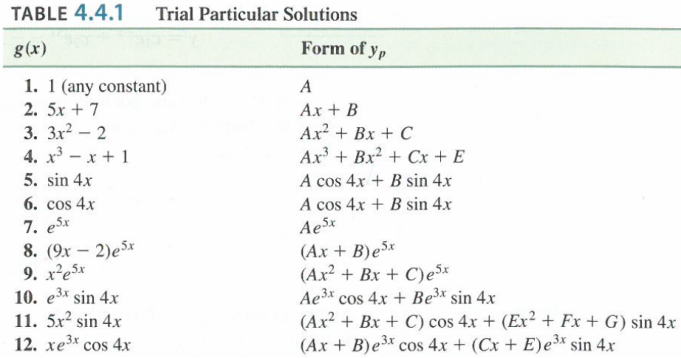
\includegraphics[width=0.55\textwidth]{figs/yptable.pdf}
\end{document}
